% ShadowVeil overview: lookahead-scheduled shadow branch (vector). 1 unit = 0.1 mm, width ~ 86 mm
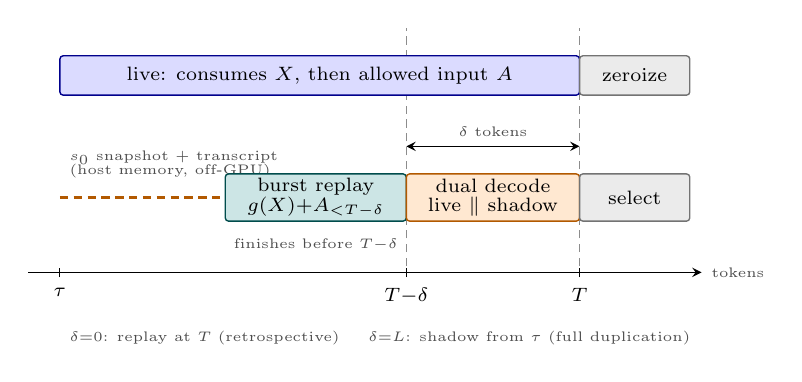
\begin{tikzpicture}[x=0.1mm,y=0.1mm,font=\scriptsize,>=stealth,
  live/.style={draw=blue!55!black,fill=blue!14,rounded corners=1.2pt,line width=0.5pt},
  shd/.style={draw=orange!70!black,fill=orange!18,rounded corners=1.2pt,line width=0.5pt},
  brs/.style={draw=teal!60!black,fill=teal!20,rounded corners=1.2pt,line width=0.5pt},
  gry/.style={draw=black!55,fill=black!8,rounded corners=1.2pt,line width=0.5pt},
  note/.style={font=\tiny,text=black!70}]
\def\xt{40}\def\xb{250}\def\xd{480}\def\xT{700}\def\xe{840}
% timeline
\draw[->,line width=0.5pt] (0,0) -- (\xe+15,0) node[right,note]{tokens};
\foreach \x/\l in {\xt/{$\tau$},\xd/{$T{-}\delta$},\xT/{$T$}}{\draw (\x,-6) -- (\x,6) node[below=4pt] {\l};}
\draw[densely dashed,black!45] (\xd,8) -- (\xd,310);
\draw[densely dashed,black!45] (\xT,8) -- (\xT,310);
% live branch
\draw[live] (\xt,225) rectangle (\xT,275);
\node at (370,250) {live: consumes $X$, then allowed input $A$};
\draw[gry] (\xT,225) rectangle (\xe,275);
\node at (770,250) {zeroize};
% shadow branch
\draw[densely dashed,orange!70!black,line width=0.8pt] (\xt,95) -- (\xb,95);
\node[note,anchor=south west,align=left] at (\xt,108) {$s_0$ snapshot $+$ transcript\\[-1pt](host memory, off-GPU)};
\draw[brs] (\xb,65) rectangle (\xd,125);
\node[align=center] at (365,95) {burst replay\\[-1pt]$g(X){+}A_{<T-\delta}$};
\draw[shd] (\xd,65) rectangle (\xT,125);
\node[align=center] at (590,95) {dual decode\\[-1pt]live $\Vert$ shadow};
\draw[gry] (\xT,65) rectangle (\xe,125);
\node at (770,95) {select};
\draw[<->,line width=0.5pt] (\xd,160) -- (\xT,160) node[midway,above,note]{$\delta$ tokens};
\node[note,anchor=north,align=center] at (365,55) {finishes before $T{-}\delta$};
\node[note,anchor=north west] at (\xt,-62) {$\delta{=}0$: replay at $T$ (retrospective) \hspace{2mm} $\delta{=}L$: shadow from $\tau$ (full duplication)};
\end{tikzpicture}
